\documentclass{standalone}
\usepackage{tikz}

\begin{document}

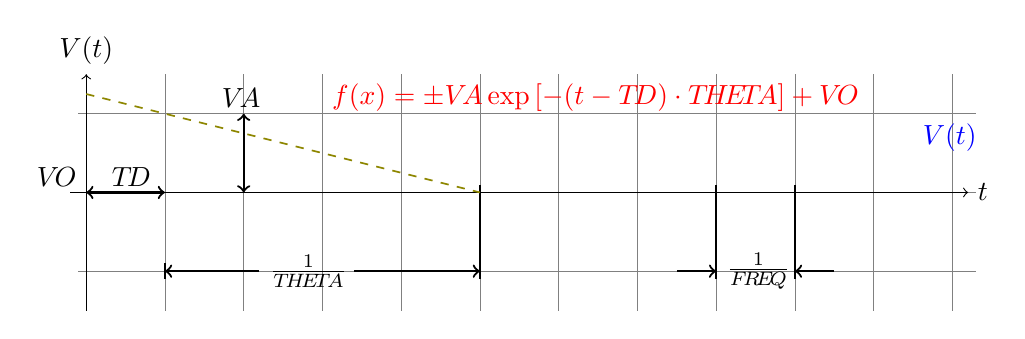
\begin{tikzpicture}[domain=0:11]
    \draw[very thin,color=gray] (-0.1,-1.5) grid (11.3,1.5);
    \draw[->] (-0.2,0) -- (11.2,0) node[right] {$t$};
    \draw[->] (0,-1.5) -- (0,1.5) node[above] {$V(t)$};
    \draw[dashed, color=red] plot[id=exp] function{exp((-x+1)*.25)} 
       node[right] {};
     \draw[dashed, color=red] plot[id=exp] function{-exp((-x+1)*.25)} 
       node[right] {};
         \draw[color=red] (3, 1.2)
       node[right] {$f(x) =\pm V\!A \exp \left[-(t-T\!D)\cdot T\!H\!E\!T\!A\right] + V\!O$};
    \draw[color=blue, semithick] plot[id=sin, samples=1000] function{sin((x-1)*2*pi/5*5)*(x>=1 ? 1 : 0)*exp((-x+1)*.25)} 
        node[right] {};
    \draw[thick, <->] (0,0) -- (1,0) node[] {};
    \draw[thick, <->] (2,0) -- (2,1) node[] {};
    \draw[] (.2,.2) node[right] {$T\!D$};
    \draw[] (1.6,1.2) node[right] {$V\!A$};
    \draw[] (0,.2) node[left] {$V\!O$};
    \draw[thick, ->] (7.5,-1) -- (8,-1) node[right] {$\frac{1}{F\!R\!E\!Q}$};
    \draw[thick, <-] (9,-1) -- (9.5,-1) node[] {};
    \draw[semithick, -] (9,-1.1) -- (9,0.1) node[] {};
    \draw[semithick, -] (8,-1.1) -- (8,0.1) node[] {};
    \draw[semithick, -] (1,-1.1) -- (1,-.9) node[] {};
    \draw[semithick, -] (5,-1.1) -- (5,0.1) node[] {};
    \draw[thick, <-] (1,-1) -- (2.2,-1) node[right] {$\frac{1}{T\!H\!E\!T\!A}$};
    \draw[thick, ->] (3.4,-1) -- (5,-1) node[] {};
    \draw[color=blue] (10.5,.7) node[right] {$V(t)$};
        \draw[dashed, color=olive, semithick] (0,1.25) -- (5,0) node[] {};

\end{tikzpicture}

\end{document}
